\documentclass[11pt,a4paper]{article}

% ---------------------------------------------------------------------------
% Global production optima and the sharp positive-response capacity of
% autocatalytic networks.
%
% Author metadata: set the three macros below before submission.
% They are deliberately left blank in this version.
% ---------------------------------------------------------------------------
\newcommand{\PaperAuthor}{}
\newcommand{\PaperAffiliation}{}
\newcommand{\PaperDate}{14 September 2026}
% Author of the companion manuscript in refs.bib; replace by the author list.
\newcommand{\CompanionAuthor}{Anonymous}

\usepackage[T1]{fontenc}
\usepackage[utf8]{inputenc}
\usepackage{lmodern}
\usepackage{microtype}
\usepackage[a4paper,margin=1.05in]{geometry}
\usepackage{amsmath,amssymb,amsthm,mathtools}
\usepackage{booktabs}
\usepackage{array}
\usepackage{enumitem}
\usepackage{xcolor}
\usepackage{graphicx}
\usepackage{tikz}
\usetikzlibrary{arrows.meta,positioning,calc}
\usepackage{listings}
\usepackage[obeyspaces,spaces]{url}
\usepackage[numbers,sort&compress]{natbib}
\usepackage[colorlinks=true,linkcolor=blue!55!black,citecolor=blue!55!black,urlcolor=blue!55!black]{hyperref}
\hypersetup{pdftitle={Global production optima and the sharp positive-response capacity of autocatalytic networks},
  pdfkeywords={autocatalysis, mass action, global optimum, thermodynamic affinity, response capacity, chemical reaction networks, Lean}}

\DeclareUrlCommand\lean{\urlstyle{tt}}
\setlist{itemsep=2pt,topsep=3pt}
\setlength{\emergencystretch}{1.5em}
\graphicspath{{figures/}}

\lstdefinelanguage{Lean}{
  morekeywords={theorem,def,structure,inductive,namespace,end,import,by,intro,exact,constructor,refine,where,abbrev,noncomputable},
  sensitive=true,
  morecomment=[l]{--},
  morestring=[b]",
}
\lstset{
  language=Lean,
  basicstyle=\ttfamily\small,
  keywordstyle=\bfseries,
  commentstyle=\itshape\color{black!60},
  columns=fullflexible,
  keepspaces=true,
  breaklines=true,
  frame=single,
  framerule=0.3pt,
  xleftmargin=1em,
  xrightmargin=1em,
  extendedchars=true,
  literate={≤}{{$\le$}}1 {≥}{{$\ge$}}1 {ℕ}{{$\mathbb{N}$}}1 {ℝ}{{$\mathbb{R}$}}1 {→}{{$\to$}}1 {∀}{{$\forall$}}1 {∃}{{$\exists$}}1 {≠}{{$\neq$}}1 {∧}{{$\wedge$}}1 {¬}{{$\neg$}}1 {↔}{{$\leftrightarrow$}}1 {∑}{{$\sum$}}1 {∏}{{$\prod$}}1 {₀}{{$_0$}}1 {₁}{{$_1$}}1 {₂}{{$_2$}}1 {ᵀ}{{$^{\mathsf T}$}}1 {⁻¹}{{$^{-1}$}}1 {•}{{$\cdot$}}1 {λ}{{$\lambda$}}1 {ε}{{$\varepsilon$}}1 {⟨}{{$\langle$}}1 {⟩}{{$\rangle$}}1 {∈}{{$\in$}}1 {∅}{{$\emptyset$}}1 {·}{{$\cdot$}}1 {ι}{{$\iota$}}1
}

\theoremstyle{plain}
\newtheorem{theorem}{Theorem}[section]
\newtheorem{proposition}[theorem]{Proposition}
\newtheorem{lemma}[theorem]{Lemma}
\newtheorem{corollary}[theorem]{Corollary}
\theoremstyle{definition}
\newtheorem{definition}[theorem]{Definition}
\newtheorem{assumption}[theorem]{Standing assumptions}
\newtheorem{example}[theorem]{Example}
\theoremstyle{remark}
\newtheorem{remark}[theorem]{Remark}

\numberwithin{equation}{section}

\newcommand{\R}{\mathbb{R}}
\newcommand{\N}{\mathbb{N}}
\newcommand{\T}{\mathsf{T}}
\newcommand{\Sp}{S_{+}}
\newcommand{\Sm}{S_{-}}
\newcommand{\one}{\mathbf{1}}
\newcommand{\cone}{\mathcal{F}}
\newcommand{\fiber}{\mathcal{M}}
\newcommand{\Vresp}{\mathcal{V}_{\mathrm{resp}}}
\newcommand{\Vloc}{\mathcal{V}_{\mathrm{loc}}}
\newcommand{\Vglob}{\mathcal{V}_{\mathrm{glob}}}
\newcommand{\Vuniq}{\mathcal{V}_{\mathrm{uniq}}}
\newcommand{\eps}{\varepsilon}
\newcommand{\Diag}{\operatorname{diag}}
\newcommand{\Ker}{\operatorname{ker}}
\newcommand{\Jmin}{J_{\min}}
\newcommand{\Jmax}{J_{\max}}
\newcommand{\Dint}{D_{\mathrm{int}}}
\renewcommand{\odot}{\circ}

\title{Global production optima and the sharp positive-response capacity of autocatalytic networks}
\author{\PaperAuthor\\ \small \PaperAffiliation}
\date{\PaperDate}

\begin{document}
\maketitle

\begin{abstract}
For a tightly coupled mass-action autocatalytic network whose stationary production of a controlled species is maximal, the affinity of the overall reaction is determined by the first-order response of the one-way fluxes to the control. Despons, De~Decker and Lacoste used this identity to constrain the optimal affinity by network structure, and a companion paper identified the exact response-level quantity, the capacity $L(T,w)$ of the forward-response cone, as the greatest lower bound of the affinity at nondegenerate local production maxima on a rooted class of square sources. What remained open is whether such a local maximum is the global one: a response profile fixes the derivative balance at a critical point but says nothing, a priori, about the rest of the positive stationary set of the nonlinear source. We close this gap. For square reversible mass-action sources with invertible reactant and net stoichiometric matrices, one controlled species, a positive production mode and a nonnegative response matrix $T=\Sp^{-1}\Sm$, every positive forward-response profile is realized by positive rate constants at a state that maximizes production over the entire positive stationary set, in every component. The proof has two ingredients: in reaction log-coordinates the stationary equations reduce to a common normalized current for every reaction, and at the reaction minimizing the response-scaled log-coordinate, strict convexity of the exponential and nonnegativity of $T$ bound that current by one. Rootedness of the response digraph is not needed for the bound; it enters only through the regular local realization, so the response, regular-local and regular-global affinity value sets coincide, including their unattained infima. Strong connectivity, or more generally a linear subcriticality certificate on each transient strong component, makes the maximizer unique. A worked rooted source with exactly two global maximizers shows that rootedness alone does not, and that a positive stationary current does not imply a positive forward response. The same normalization shows that prescribing effective equilibrium constants leaves every capacity unchanged when reference activities are free, and turns the affinity into an exact statement about the controlled activity relative to its equilibrium value. Reverse one-way flux budgets at a required output give an exact linear feasibility condition, and a two-reaction recycling family yields closed-form production--turnover trade-offs, an inverse-gap turnover cost near capacity, and a controlled operating point that is globally attracting. The global comparison, the uniqueness theorem and the capacity equalities are verified in Lean~4 against Mathlib; the boundary of the formal scope is stated explicitly.
\end{abstract}

\section{Introduction}\label{sec:intro}

\subsection{Optimal affinity and the response identity}
An autocatalytic network sustains the production of one of its own species when a controller maintains the activity of that species and removes the surplus. At a stationary state the production current $J$ and the thermodynamic driving force of the overall reaction, its affinity $A$, are linked, and one may ask how small the affinity can be at the operating point where the production is maximal. Despons, De~Decker and Lacoste~\citep{despons2024} showed that at such an optimum the affinity is determined by the first-order response of the one-way fluxes to the control, and used the identity to derive structural constraints on the optimal affinity and on the controlled concentration; their setting is the thermodynamically consistent mass-action framework of open chemical networks~\citep{polettini2014,rao2016}, applied to the autocatalytic cores classified in~\citep{blokhuis2020,unterberger2022,nandan2026}. The response framework is attractive because it uses only the complexes and the control, not the kinetic parameters, and because it isolates the driving force that the chemistry must supply from the rest of the operating cost.

A companion paper~\citep{companion2026} refuted the conjectured lower bound $A^*\ge\log(\beta/\alpha)$ in terms of the gross stoichiometric amplification and replaced it by an exact response-level quantity. With $T=\Sp^{-1}\Sm$ built from the reactant and product complex matrices and $w$ the integer production mode, the \emph{capacity}
\[
L(T,w)=\inf\Big\{\prod_i\big((T^{\T}f)_i/f_i\big)^{w_i}:\ f>0,\ T^{\T}f>f\Big\}
\]
is the greatest lower bound of $e^{A^*}$ over all optima in the forward-response regime, and on a rooted class of square sources every point of the forward-response cone is the response profile of an actual positive mass-action network at a nondegenerate strict local production maximum.

That result is local. A response profile determines the derivative balance at a critical point and, through the routing structure of $T$, the regularity and curvature of the stationary branch through it. It does not by itself say anything about the other positive stationary states of the same nonlinear source, and the companion paper accordingly treated global optimality as a separate layer, proved for one two-reaction family by an explicit polynomial certificate and otherwise left open. Three distinct assertions were therefore in play: that a profile satisfies the affinity--response identity, that it is realized at a regular local maximum, and that this maximum is the global one. The present paper proves the third assertion in full generality on the nonnegative-response class, and shows that the three affinity value sets coincide.

\subsection{Main results}
Throughout, a \emph{source} consists of nonnegative complex matrices $\Sp,\Sm\in\R^{n\times n}$ with $\Sp$ and $S=\Sm-\Sp$ invertible, one controlled species $X$, positive rate constants, and a positive production mode $g=S^{-1}e_X$. The response matrix is $T=\Sp^{-1}\Sm$ and the response digraph has an edge $i\to j$ whenever $T_{ji}>0$. The forward-response cone is $\cone(T)=\{f>0:T^{\T}f>f\}$, with response ratios $q_i=(T^{\T}f)_i/f_i>1$.

\begin{enumerate}[label=(\Alph*)]
\item \emph{Global maximum principle} (Theorem~\ref{thm:global}). Let $T\ge0$ and $f\in\cone(T)$. The positive rate constants $k^-_i=J_0g_i/(q_i-1)$, $k^+_i=q_ik^-_i$ make the unit state stationary with production $J_0$, and every positive stationary state of this source, in every component of the stationary set, has production at most $J_0$. Rootedness is not needed.
\item \emph{Uniqueness} (Theorems~\ref{thm:unique} and~\ref{thm:subcritical}). If the response digraph is strongly connected, the unit state is the only global maximizer. More generally, if the digraph is rooted and every transient strong component $C$ admits a vector $b_C>0$ with $T_{CC}b_C\le b_C$, the maximizer is unique.
\item \emph{Arbitrary reference points} (Corollary~\ref{cor:arbitrary}). For a source with arbitrary positive rates, every positive stationary state at which the one-way flux ratios equal the response ratios of some profile in the cone is a global production maximizer; in particular every regular positive-production critical point in the forward regime is global.
\item \emph{Sharp global capacity} (Theorem~\ref{thm:capacity}). If the response digraph is rooted and the cone is nonempty, the sets of affinity products attained at forward-response profiles, at regular nondegenerate strict local maxima, and at regular global maxima coincide, so their infima are all equal to $L(T,w)$; under strong connectivity the same holds for unique global maxima. The infimum need not be attained, and every value within $\eps$ of it is realized at a regular global maximum.
\item \emph{Fixed thermodynamics and turnover budgets} (Propositions~\ref{prop:fixedK} and~\ref{prop:budget}). Prescribing the effective equilibrium constants leaves all value sets unchanged when reference activities are free, and gives the exact identity $\log\Phi_w=N\log(z_{\mathrm{eq},X}/z^*_X)$ between the affinity and the ratio of equilibrium to operating activity of the controlled species. Requiring production at least $\Jmin$ with reverse one-way fluxes at most $\beta_i$ restricts the cone to an explicit polyhedral subcone, with exact rational feasibility certificates.
\item \emph{Two exact examples} (Sections~\ref{sec:recycling} and~\ref{sec:rooted}). A recycling family gives closed-form production--turnover trade-offs, the inverse-gap cost $v_1^-/J=(1-1/m)/(\Phi-L)$ of approaching capacity, and a globally attracting controlled operating point. A rooted but not strongly connected source has exactly two global maximizers, only one of which has a positive forward response; it shows that the hypotheses of (B) cannot be dropped and that the positive-response capacity is a statement about responses, not about positive currents.
\end{enumerate}

\subsection{What is new relative to the companion paper}
The companion paper proved the regular local realization on a class of sources defined by nonnegativity of $T$, rootedness of the response digraph, and an accessibility condition on the cone. Three things change here. First, global optimality is no longer a separate layer needing an independent certificate: on the nonnegative class the response data $(T,q)$ determine the normalized stationary equations completely, and a one-line comparison at a response-scaled minimum bounds every stationary state (Section~\ref{sec:global}). The companion paper's caveat that global optimality needs information beyond the response profile therefore does not apply within this class; what remains source dependent are concentration coordinates and dynamical stability, not the value of the maximal production. Second, the accessibility condition is a consequence of the positive production mode (Lemma~\ref{lem:access}), so the class is described by nonnegativity of $T$ and rootedness alone. Third, the local realization itself is not used for the upper bound, only for the existence of a regular branch; the bound holds for every $f\in\cone(T)$ and $T\ge0$, rooted or not.

\subsection{Formal verification}
The global comparison, the equality propagation, the value-set and capacity identities, the near-capacity realization, and the arbitrary-reference comparison are compiled in Lean~4~\citep{demoura2021} against Mathlib~\citep{mathlib2020} with warnings treated as errors, on top of the companion paper's compiled local-realization theorem. A separate module verifies the algebraic identities behind the operating consequences of Sections~\ref{sec:thermo}--\ref{sec:recycling}. Section~\ref{sec:formal} lists the root declarations, the correspondence between the theorems of this paper and the compiled statements, and the steps that are proved conventionally: the subcritical-block uniqueness theorem, the derivative-balance step of Corollary~\ref{cor:arbitrary}, the transfer of regularity under fixed equilibrium constants, the constrained-capacity corollary, the convergence of the controlled ODE, and the rooted counterexample.

\subsection{Organisation and conventions}
Section~\ref{sec:setting} fixes the setting and the normalized reconstruction. Section~\ref{sec:global} proves the global maximum principle and the uniqueness theorems. Section~\ref{sec:capacity} combines them with the local realization into the capacity theorem. Section~\ref{sec:thermo} treats prescribed equilibrium constants and turnover budgets, Section~\ref{sec:recycling} the recycling family, and Section~\ref{sec:rooted} the rooted obstruction. Section~\ref{sec:discussion} discusses scope and open problems and Section~\ref{sec:formal} the formal development. Vectors are columns, $\one$ is the all-ones vector, $\odot$ is the entrywise product, $\Diag(v)$ the diagonal matrix, and inequalities between vectors are entrywise. Activities are dimensionless relative to fixed standard states; $RT=1$. We write $\Sp,\Sm$ for the reactant and product complex matrices as in~\citep{companion2026}; other authors write $A,B$.

\section{Setting}\label{sec:setting}

\subsection{Sources, control and tight coupling}
Let $n\ge1$. A source has $n$ species and $n$ reversible reactions. Columns of the nonnegative matrices $\Sp,\Sm\in\R^{n\times n}_{\ge0}$ are the reactant and product complexes; in applications the entries are integers, and the results below use only nonnegativity. Species $X$ is controlled: its activity $z_X$ is maintained externally and the controller absorbs the net production. For an activity vector $z\in\R^n_{>0}$ write $\zeta=\log z$ entrywise. The mass-action one-way fluxes and net currents are~\citep{hornjackson1972,feinberg2019}
\begin{equation}\label{eq:massaction}
 j^\pm_i(z)=k^\pm_i\,z^{(S_\pm)_i}=k^\pm_i\exp\big((S_\pm^{\T}\zeta)_i\big),\qquad j_i=j^+_i-j^-_i,
\end{equation}
where $(S_\pm)_i$ is the $i$th column and $z^{a}=\prod_\sigma z_\sigma^{a_\sigma}$. Fixed food and waste activities are absorbed into the effective coefficients $k^\pm$, as in~\citep{despons2024}.

\begin{assumption}\label{ass:standing}
$\Sp$ and $S\coloneqq\Sm-\Sp$ are invertible; the \emph{production mode} $g\coloneqq S^{-1}e_X$ is positive; the \emph{response matrix}
\begin{equation}\label{eq:T}
 T\coloneqq\Sp^{-1}\Sm,\qquad \Sm=\Sp T,
\end{equation}
is entrywise nonnegative. A weight vector $w\in\N^n$ is fixed; for thermodynamic statements $w=Ng$ with $N>0$.
\end{assumption}

The stationary set (the \emph{fiber}) and the controlled production are
\begin{equation}\label{eq:fiber}
 \fiber=\{z>0:\ (Sj(z))_s=0\ \text{for } s\ne X\},\qquad J(z)=(Sj(z))_X .
\end{equation}
Since $S$ is invertible and $Sg=e_X$, the fiber is characterized by \emph{tight coupling}~\citep[Eq.~(21)]{despons2024}:
\begin{equation}\label{eq:tight}
 z\in\fiber\quad\Longleftrightarrow\quad j(z)=J(z)\,g .
\end{equation}
Nothing in the definition restricts $\fiber$ to a neighbourhood of any state or to a single connected component.

\subsection{Response profiles, affinity and capacity}
Suppose $\fiber$ is a smooth curve near $z^*$, parametrized by $s=\log z_X$, with logarithmic tangent $u=d\zeta/ds$ at $z^*$, so $u_X=1$. Differentiating~\eqref{eq:massaction},
\begin{equation}\label{eq:fh}
 f\coloneqq\Sp^{\T}u,\qquad h\coloneqq\Sm^{\T}u=T^{\T}f
\end{equation}
are the forward and reverse response profiles~\citep[Eq.~(26)]{despons2024}. At a zero-derivative critical point of $J$ with $J>0$, tight coupling gives $\dot j=\dot Jg=0$, hence the \emph{derivative balance} $j^+_if_i=j^-_ih_i$; in the \emph{forward regime} $f>0$ this reads $j^+_i/j^-_i=h_i/f_i$~\citep[Eqs.~(27)--(30)]{despons2024}. Define
\begin{equation}\label{eq:cone}
 \cone(T)\coloneqq\{f>0:\ T^{\T}f>f\},\qquad q_i(f)\coloneqq\frac{(T^{\T}f)_i}{f_i}>1 .
\end{equation}
Positive net currents and positive forward responses are different conditions; Section~\ref{sec:rooted} separates them.

The affinity of reaction $i$ is $\log(j^+_i/j^-_i)$ and the affinity per unit production along the mode $g$ is $\mathcal A_g=\sum_ig_i\log(j^+_i/j^-_i)$; the reaction dissipation at a stationary state is $J\mathcal A_g$~\citep{polettini2014,rao2016}. With $w=Ng$,
\begin{equation}\label{eq:affinity}
 \Phi_w(f)\coloneqq\prod_iq_i(f)^{w_i},\qquad e^{N\mathcal A_g}=\Phi_w(f)\ \text{at a forward-regime critical point},
\end{equation}
by derivative balance. The \emph{capacity}~\citep{companion2026} is
\begin{equation}\label{eq:capacity}
 L(T,w)\coloneqq\inf_{f\in\cone(T)}\Phi_w(f)\qquad(\inf\emptyset\coloneqq0).
\end{equation}
Both $\cone(T)$ and $\Phi_w$ are invariant under positive rescaling of $f$; $\Phi_w\ge1$ on the cone. This is the optimization problem of~\citep[Supplementary Note~11]{despons2024} in response coordinates; what is proved below is its exact relation to actual global optima.

\subsection{The response digraph}
The \emph{response digraph} $G(T)$ has vertex set $\{1,\dots,n\}$ and an edge $i\to j$ exactly when $T_{ji}>0$. It is \emph{rooted} if some vertex is reachable from every vertex by a directed path (of length zero allowed); equivalently it has exactly one terminal strong component. It is \emph{strongly connected} if every vertex is reachable from every other. A strong component is \emph{transient} if it is not terminal. For a set $C$ of vertices, $T_{CC}$ denotes the principal submatrix on $C$.

\subsection{The normalized reconstruction}
Fix $f\in\cone(T)$, write $q=q(f)$, and choose a current scale $J_0>0$. The \emph{normalized reconstruction} is the source with the same complexes and control and rate constants
\begin{equation}\label{eq:rates}
 k^-_i\coloneqq\frac{J_0g_i}{q_i-1},\qquad k^+_i\coloneqq q_ik^-_i=\frac{J_0g_iq_i}{q_i-1}.
\end{equation}
These are positive, $k^+-k^-=J_0g$, and $k^+\odot f=k^-\odot h$. At the unit state $z=\one$ every monomial equals one, so $j(\one)=J_0g$: by~\eqref{eq:tight}, $\one\in\fiber$ and $J(\one)=J_0$, and the derivative balance holds there with profiles $(f,h)$~\citep[Lemma~5.2]{companion2026}.

\begin{lemma}[Normalized currents]\label{lem:normalized}
Let $\xi\coloneqq\Sp^{\T}\zeta$ be the reaction log-coordinates of $z=e^{\zeta}$. The map $z\mapsto\xi$ is a bijection of $\R^n_{>0}$ onto $\R^n$, $\Sm^{\T}\zeta=T^{\T}\xi$, and the currents of the reconstruction~\eqref{eq:rates} satisfy
\begin{equation}\label{eq:normalized}
 C_i(\xi)\coloneqq\frac{j_i(z)}{J_0g_i}=\frac{q_ie^{\xi_i}-e^{(T^{\T}\xi)_i}}{q_i-1}.
\end{equation}
If $z\in\fiber$, then $C_i(\xi)=t$ for every $i$, where $t=J(z)/J_0$.
\end{lemma}
\begin{proof}
Bijectivity is invertibility of $\Sp^{\T}$, and $\Sm^{\T}\zeta=T^{\T}\Sp^{\T}\zeta=T^{\T}\xi$ by~\eqref{eq:T}. Then $j^+_i=k^+_ie^{\xi_i}$ and $j^-_i=k^-_ie^{(T^{\T}\xi)_i}$, and dividing by $J_0g_i$ gives~\eqref{eq:normalized}. On the fiber, $j=J(z)g$ by~\eqref{eq:tight}, so $C_i=J(z)/J_0$ for all $i$.
\end{proof}

Lemma~\ref{lem:normalized} is the whole point of the normalization: the response data $(T,q)$ determine the stationary equations $C_i(\xi)=t$ of the reconstruction on all of $\R^n_{>0}$, not only their linearization at $\one$.

\section{The global maximum principle}\label{sec:global}

\subsection{Two elementary inequalities}

\begin{lemma}[Scalar tangent gap]\label{lem:scalar}
For $q>1$ and $a\in\R$,
\begin{equation}\label{eq:scalar}
 e^{qa}-qe^{a}+q-1\ \ge\ 0,\qquad\text{with equality if and only if }a=0 .
\end{equation}
\end{lemma}
\begin{proof}
Write $a=q^{-1}(qa)+(1-q^{-1})\cdot0$. Strict convexity of the exponential gives $e^{a}\le q^{-1}e^{qa}+(1-q^{-1})$, with equality only if $qa=0$. Multiply by $q$.
\end{proof}

\begin{lemma}[Minimum comparison]\label{lem:minimum}
Let $T\ge0$, $f>0$, $q=q(f)$, and $\xi\in\R^n$. Choose $k$ minimizing $\xi_i/f_i$ over $i$. Then
\begin{equation}\label{eq:minimum}
 (T^{\T}\xi)_k=\sum_jT_{jk}f_j\frac{\xi_j}{f_j}\ \ge\ \frac{\xi_k}{f_k}\sum_jT_{jk}f_j=q_k\xi_k ,
\end{equation}
and consequently, for the normalized currents~\eqref{eq:normalized} with $q>1$,
\begin{equation}\label{eq:bottleneck}
 C_k(\xi)\ \le\ \frac{q_ke^{\xi_k}-e^{q_k\xi_k}}{q_k-1}\ \le\ 1 .
\end{equation}
\end{lemma}
\begin{proof}
Each term $T_{jk}f_j\ge0$ and $\xi_j/f_j\ge\xi_k/f_k$, which gives~\eqref{eq:minimum}; the last equality is the definition of $q_k$. Since the exponential is increasing, $e^{(T^{\T}\xi)_k}\ge e^{q_k\xi_k}$, which gives the first inequality in~\eqref{eq:bottleneck}, and the second is Lemma~\ref{lem:scalar}.
\end{proof}

Lemma~\ref{lem:minimum} does not assume stationarity: at \emph{every} positive state of the reconstruction, the reaction that minimizes $\xi_i/f_i$ carries at most its reference current. The two inequalities in~\eqref{eq:bottleneck} have an exact deficit. With $\delta_k\coloneqq(T^{\T}\xi)_k-q_k\xi_k\ge0$,
\begin{equation}\label{eq:gap}
 1-C_k(\xi)=\frac{\big(e^{q_k\xi_k}-q_ke^{\xi_k}+q_k-1\big)+e^{q_k\xi_k}\big(e^{\delta_k}-1\big)}{q_k-1},
\end{equation}
a sum of the scalar tangent gap and a routing gap, both nonnegative at the selected index. Individual reactions at other indices may exceed their reference currents off the fiber; the selected bottleneck reaction cannot.

\subsection{Global domination}

\begin{theorem}[Global production maximum]\label{thm:global}
Under Assumptions~\ref{ass:standing}, let $f\in\cone(T)$ and $J_0>0$. For the normalized reconstruction~\eqref{eq:rates},
\[
 J(z)\le J_0\qquad\text{for every }z\in\fiber .
\]
Thus $\one$ is a global production maximizer over the entire positive stationary set. Rootedness of $G(T)$ is not needed.
\end{theorem}
\begin{proof}
Let $z\in\fiber$ with reaction log-coordinates $\xi$. By Lemma~\ref{lem:normalized}, $C_i(\xi)=t\coloneqq J(z)/J_0$ for every $i$. By Lemma~\ref{lem:minimum}, $t=C_k(\xi)\le1$.
\end{proof}

\begin{remark}[A bottleneck reading]\label{rem:bottleneck}
Since Lemma~\ref{lem:minimum} holds off the fiber, Theorem~\ref{thm:global} has a purely algebraic form: for the reconstruction~\eqref{eq:rates},
\[
 \max_{z>0}\ \min_i\ \frac{j_i(z)}{g_i}=J_0,
\]
attained at $\one$. Sustained physical production also requires the stationarity conditions, which is why the theorem is stated on $\fiber$; but the bound is a property of the currents themselves.
\end{remark}

\begin{remark}[Why the proof is short]
The argument does not eliminate the stationary equations, does not continue a branch, and is uniform in $n$: it compares one scalar quantity at one index. What makes it possible is that in reaction log-coordinates the reconstruction's currents are \emph{exactly} the two-exponential expressions~\eqref{eq:normalized} with fixed data $(T,q)$. Earlier attempts at global statements in this setting treated higher-order behaviour as more flexible than fixed monomial kinetics permits; the same-response search for a globality separation is closed by Lemma~\ref{lem:normalized}.
\end{remark}

\subsection{Uniqueness}

\begin{lemma}[The equality set]\label{lem:equality}
In the setting of Theorem~\ref{thm:global}, let $z\in\fiber$ with $J(z)=J_0$ and let $\xi$ be its reaction log-coordinates. Then $\xi\ge0$, $\xi_k=0$ at any index $k$ minimizing $\xi_i/f_i$, and zeros propagate along edges of $G(T)$: if $\xi_i=0$ and $T_{ji}>0$ then $\xi_j=0$.
\end{lemma}
\begin{proof}
Here $t=1$, so both inequalities in~\eqref{eq:bottleneck} are equalities at $k$. The second forces $\xi_k=0$ by Lemma~\ref{lem:scalar}. By minimality of $\xi_k/f_k=0$, every $\xi_i\ge0$. If $\xi_i=0$, the equation $C_i(\xi)=1$ gives $q_i-e^{(T^{\T}\xi)_i}=q_i-1$, so $(T^{\T}\xi)_i=\sum_jT_{ji}\xi_j=0$; every summand is nonnegative, hence $\xi_j=0$ whenever $T_{ji}>0$.
\end{proof}

\begin{theorem}[Unique global maximum under strong connectivity]\label{thm:unique}
If, in addition, $G(T)$ is strongly connected, then $J(z)=J_0$ for $z\in\fiber$ only at $z=\one$.
\end{theorem}
\begin{proof}
By Lemma~\ref{lem:equality}, $\xi_k=0$ and zeros propagate along edges. Every vertex is reachable from $k$, so $\xi=0$, and invertibility of $\Sp^{\T}$ gives $\zeta=0$, $z=\one$.
\end{proof}

Strong connectivity is a source-checkable sufficient condition, not a necessary one: the companion paper's power family has unique global maxima with a reducible rooted digraph. The following extension covers such cases by a finite linear certificate on each transient component.

\begin{theorem}[Uniqueness with subcritical transient components]\label{thm:subcritical}
Suppose $G(T)$ is rooted and that every transient strong component $C$ admits a vector $b_C\in\R^C_{>0}$ with
\begin{equation}\label{eq:subcritical}
 T_{CC}\,b_C\le b_C .
\end{equation}
Then, in the setting of Theorem~\ref{thm:global}, $\one$ is the unique global maximizer.
\end{theorem}
\begin{proof}
Let $z\in\fiber$ with $J(z)=J_0$ and reaction log-coordinates $\xi$. By Lemma~\ref{lem:equality}, $\xi\ge0$, $\xi_k=0$ at a minimizer $k$, and zeros propagate along edges. Since $G(T)$ is rooted, some vertex of the terminal component $C_0$ is reachable from $k$; propagation along that path and then within the strongly connected set $C_0$ gives $\xi_i=0$ for all $i\in C_0$.

Now process the transient components in reverse topological order of the condensation, so that when $C$ is treated, $\xi$ already vanishes on every component reachable from $C$. For $i\in C$, every edge $i\to j$ with $T_{ji}>0$ has $j\in C$ or $j$ in a component reachable from $C$; hence
\[
 (T^{\T}\xi)_i=\sum_{j\in C}T_{ji}\xi_j=(T_{CC}^{\T}\xi_C)_i .
\]
The stationary equation $C_i(\xi)=1$ reads $e^{(T^{\T}\xi)_i}=q_ie^{\xi_i}-q_i+1$, that is,
\begin{equation}\label{eq:logform}
 (T_{CC}^{\T}\xi_C)_i-\xi_i=\log\big(q_i-(q_i-1)e^{-\xi_i}\big)\qquad(i\in C).
\end{equation}
For $\xi_i\ge0$ the argument of the logarithm lies in $[1,q_i)$, so the right side is nonnegative, and it is strictly positive when $\xi_i>0$. Suppose $\xi_C\ne0$. Pairing~\eqref{eq:logform} with $b_C>0$ gives
\[
 0<b_C^{\T}\big(T_{CC}^{\T}-I\big)\xi_C=\big(T_{CC}b_C-b_C\big)^{\T}\xi_C\le0,
\]
the last inequality because $T_{CC}b_C-b_C\le0$ and $\xi_C\ge0$. This contradiction shows $\xi_C=0$. By induction $\xi=0$, and $z=\one$.
\end{proof}

\begin{remark}\label{rem:subcritical}
For an irreducible nonnegative block, \eqref{eq:subcritical} is equivalent to spectral radius at most one~\citep{berman1994}, but the certificate form needs no spectral theory and, for rational $T$, is checkable exactly. A transient component consisting of a single vertex without a self-loop has $T_{CC}=0$ and satisfies~\eqref{eq:subcritical} trivially; this is the situation of the companion paper's power family, whose response digraph has one transient vertex feeding a terminal loop. The rooted source of Section~\ref{sec:rooted} has a transient component with block $\begin{psmallmatrix}0&2\\1&0\end{psmallmatrix}$ of spectral radius $\sqrt2$, no certificate exists, and uniqueness indeed fails there. We do not claim that~\eqref{eq:subcritical} is necessary for uniqueness.
\end{remark}

\subsection{Arbitrary reference points}

\begin{corollary}[Arbitrary rates and reference states]\label{cor:arbitrary}
Let a source satisfy Assumptions~\ref{ass:standing} with arbitrary positive rate constants, and let $z^*\in\fiber$ with $J(z^*)>0$ be such that the one-way flux ratios at $z^*$ are the response ratios of some $f\in\cone(T)$:
\begin{equation}\label{eq:ratiohyp}
 \frac{j^+_i(z^*)}{j^-_i(z^*)}=q_i(f)\qquad\text{for all }i .
\end{equation}
Then $J(z)\le J(z^*)$ for every $z\in\fiber$. If $G(T)$ is strongly connected, or satisfies the hypothesis of Theorem~\ref{thm:subcritical}, equality holds only at $z^*$. In particular, every regular zero-derivative critical point of $J$ with $J>0$ in the forward regime is a global production maximizer under these hypotheses.
\end{corollary}
\begin{proof}
Substitute $z=z^*\odot y$. Then $j^\pm_i(z)=j^\pm_i(z^*)\,y^{(S_\pm)_i}$, so in the variable $y$ the source has rate constants $k'^\pm=j^\pm(z^*)$. By~\eqref{eq:ratiohyp} and tight coupling at $z^*$, $k'^+_i=q_ik'^-_i$ and $k'^+_i-k'^-_i=J(z^*)g_i$, hence $k'^\pm$ is exactly the normalized reconstruction~\eqref{eq:rates} with $J_0=J(z^*)$. The substitution is a bijection between the positive stationary sets in $z$ and in $y$ that preserves currents and production, and maps $z^*$ to $\one$. Apply Theorems~\ref{thm:global}, \ref{thm:unique} and~\ref{thm:subcritical}. The last sentence follows because derivative balance at a forward-regime critical point is~\eqref{eq:ratiohyp} with $f=\Sp^{\T}u$.
\end{proof}

Fixing $(T,q)$ fixes the normalized stationary-current equations, so any two sources with the same complexes, control and one-way ratios at a critical point have the same stationary sets after translation of log activities and the same maximal production. This is a statement about stationary production; it does not assert equivalence of the time-dependent dynamics, and Section~\ref{sec:rooted} shows a global maximizer that is a saddle of the controlled dynamics.

\section{Regular realization and the capacity theorem}\label{sec:capacity}

\subsection{Automatic accessibility}
The companion paper's local realization required, for every $f\in\cone(T)$, that the controlled component of the common tangent $u=\Sp^{-\T}f$ be positive, so that the response ray can be scaled to $u_X=1$. Under a positive production mode this is automatic.

\begin{lemma}[Control accessibility]\label{lem:access}
For $f\in\cone(T)$ and $u=\Sp^{-\T}f$,
\begin{equation}\label{eq:access}
 u_X=(Sg)^{\T}u=g^{\T}S^{\T}u=\sum_ig_i\big((T^{\T}f)_i-f_i\big)>0 .
\end{equation}
\end{lemma}
\begin{proof}
$e_X=Sg$, $S^{\T}u=\Sm^{\T}u-\Sp^{\T}u=T^{\T}f-f$ by~\eqref{eq:fh}, and each summand is positive because $g>0$ and $f\in\cone(T)$.
\end{proof}

\subsection{Rooted regular local realization}
We restate the companion paper's local theorem in the present conventions and sketch its proof, since its ingredients (the routing matrix and its left null vector) recur in the discussion. It is compiled in Lean as part of the dependency chain of the present root (Section~\ref{sec:formal}).

\begin{theorem}[Rooted regular local realization~{\citep[Theorem~5.15]{companion2026}}]\label{thm:local}
Let Assumptions~\ref{ass:standing} hold and let $G(T)$ be rooted. For every $f\in\cone(T)$, scaled so that $u_X=1$ (Lemma~\ref{lem:access}), the fiber of the normalized reconstruction~\eqref{eq:rates} is a smooth curve through $\one$ parametrized by $\log z_X$, with logarithmic tangent $u$, and the production has a nondegenerate strict local maximum at $\one$ with $e^{N\mathcal A_g}=\Phi_w(f)$.
\end{theorem}
\begin{proof}[Sketch]
Define the \emph{routing matrix} $P_{ij}=T_{ji}f_j/(q_if_i)$. It is nonnegative, row stochastic, and has exactly the edges of $G(T)$. For a finite rooted row-stochastic matrix the fixed vectors $Pv=v$ are constant: the maximum and the minimum of $v$ each propagate along edges to a common reachable vertex~\citep{kemeny1976,seneta2006}. A stationary row $\pi^{\T}P=\pi^{\T}$ with $\pi\ge0$, $\pi\ne0$ exists. The Jacobian of the reaction currents with respect to $\zeta$ at $\one$ is
\[
 M=\Diag(k^-)\big(\Diag(q)-T^{\T}\big)\Sp^{\T}=\Diag(k^-_iq_if_i)\,(I-P)\,\Diag(f_i^{-1})\,\Sp^{\T},
\]
so $\Ker M=\R u$, and $\lambda_i\coloneqq\pi_i/(k^-_iq_if_i)$ gives $\lambda\ge0$, $\lambda\ne0$, $\lambda^{\T}M=0$ and $\lambda^{\T}g>0$. The noncontrolled stationary Jacobian is injective on variations $v$ with $v_X=0$: if $(SMv)_s=0$ for $s\ne X$ then $Mv=ag$ by invertibility of $S$; pairing with $\lambda$ forces $a=0$, so $v\in\R u$, and $v_X=0$ forces $v=0$. The implicit function theorem gives the branch. Differentiating $j=Jg$ along it once gives $J'(0)=0$ and tangent $u$; differentiating twice and pairing with $\lambda$ gives
\begin{equation}\label{eq:curvature}
 J''(0)=-\frac{\sum_i\lambda_ik^-_iq_i(q_i-1)f_i^2}{\lambda^{\T}g}<0 .
\end{equation}
The affinity identity is the derivative balance at $\one$.
\end{proof}

\subsection{Value sets and the capacity theorem}
Fix $(\Sp,\Sm,X,w)$ and let the positive rate constants and reference states vary over all sources with these complexes and control.

\begin{definition}[Value sets]\label{def:valuesets}
Let $\Vresp$ be the set of values $\Phi_w(f)$, $f\in\cone(T)$. Let $\Vloc$ be the set of values $e^{N\mathcal A_g}$ at regular nondegenerate strict local production maxima in the forward regime. Let $\Vglob\subseteq\Vloc$ be the subset of those that also maximize production over the entire positive fiber, ties allowed, and $\Vuniq\subseteq\Vglob$ the subset with a unique global maximizer.
\end{definition}

By definition and the response identity~\eqref{eq:affinity},
\begin{equation}\label{eq:chain}
 \Vuniq\subseteq\Vglob\subseteq\Vloc\subseteq\Vresp .
\end{equation}

\begin{theorem}[Sharp global positive-response capacity]\label{thm:capacity}
Let Assumptions~\ref{ass:standing} hold, let $G(T)$ be rooted, and let $\cone(T)\ne\emptyset$. Then
\begin{equation}\label{eq:valueeq}
 \Vglob=\Vloc=\Vresp,\qquad \inf\Vglob=\inf\Vloc=L(T,w).
\end{equation}
If $G(T)$ is strongly connected, or satisfies the hypothesis of Theorem~\ref{thm:subcritical}, then also $\Vuniq=\Vresp$ and $\inf\Vuniq=L(T,w)$.
\end{theorem}
\begin{proof}
Let $f\in\cone(T)$ and $J_0>0$. Scaling $f$ so that $u_X=1$ changes neither $q$ nor $\Phi_w$. Theorem~\ref{thm:local} realizes $\Phi_w(f)$ at a regular nondegenerate strict local maximum of the reconstruction, Theorem~\ref{thm:global} makes it global, and Theorem~\ref{thm:unique} or~\ref{thm:subcritical} makes it unique when applicable. Hence $\Vresp\subseteq\Vglob$ (and $\Vresp\subseteq\Vuniq$ in the second case), which with~\eqref{eq:chain} gives the equalities of sets; the sets are nonempty, so their infima agree.
\end{proof}

\begin{corollary}[Near-capacity realization]\label{cor:near}
Under the hypotheses of Theorem~\ref{thm:capacity}, for every $\eps>0$ there is $f_\eps\in\cone(T)$ realized at a regular global production maximum of a positive mass-action source with the given complexes and control, with
\begin{equation}\label{eq:epsilon}
 L(T,w)\le\Phi_w(f_\eps)<L(T,w)+\eps .
\end{equation}
\end{corollary}
\begin{proof}
$\Vresp$ is nonempty and bounded below by one, so the greatest-lower-bound property gives $f_\eps$; apply Theorem~\ref{thm:capacity}.
\end{proof}

No minimizer of $\Phi_w$ is assumed, and none need exist: in the recycling family of Section~\ref{sec:recycling} the capacity is approached along interior profiles but the limiting profile lies on the boundary of the cone, where a reaction ratio tends to one and the reconstruction~\eqref{eq:rates} has no positive-rate meaning. Corollary~\ref{cor:near} is the correct sharpness statement. As observed in~\citep[Remark~5.19]{companion2026}, the apparent divergence of $k^-_i$ as $q_i\downarrow1$ is a gauge effect of the free current scale $J_0$ and not of the response ray: choosing $J_0=\min\{1,\min_i(q_i-1)\}$ gives $0<k^-_i\le g_i$ and $k^+_i\le2g_i$ along any sequence, at the price of production tending to zero. Bounded one-way rates at a \emph{fixed} output are a different requirement, and Section~\ref{sec:thermo} quantifies it.

\begin{table}[t]
\centering\small
\begin{tabular}{@{}lll@{}}
\toprule
Hypotheses on the source & Conclusion & Where \\
\midrule
$T\ge0$, $g>0$, $f\in\cone(T)$ & $\one$ globally maximal, ties allowed & Thm.~\ref{thm:global} \\
$\ldots$ and $G(T)$ strongly connected & $\one$ the unique global maximizer & Thm.~\ref{thm:unique} \\
$\ldots$ and $G(T)$ rooted with certificates~\eqref{eq:subcritical} & $\one$ the unique global maximizer & Thm.~\ref{thm:subcritical} \\
$T\ge0$, $g>0$, $G(T)$ rooted & regular strict local maximum at $\one$ & Thm.~\ref{thm:local} \\
$T\ge0$, $g>0$, $G(T)$ rooted, $\cone\ne\emptyset$ & $\Vglob=\Vloc=\Vresp$, common infimum $L$ & Thm.~\ref{thm:capacity} \\
$\ldots$ strongly connected or certified & $\Vuniq=\Vresp$ & Thm.~\ref{thm:capacity} \\
\bottomrule
\end{tabular}
\caption{Which hypothesis buys which conclusion. Rootedness enters only through the regular branch; the upper bound needs none of the graph conditions.}
\label{tab:hyp}
\end{table}

\section{Fixed thermodynamics and turnover budgets}\label{sec:thermo}

\subsection{Prescribed effective equilibrium constants}
The reconstruction~\eqref{eq:rates} chooses the ratio $k^+_i/k^-_i=q_i$ freely. In a fixed thermodynamic environment the effective equilibrium constants $K_i=k^+_i/k^-_i$ are prescribed by the standard free energies of the reactions and the fixed food and waste activities. The freedom to choose ratios is not needed if the reference activities can move instead.

\begin{proposition}[Fixed-equilibrium realization]\label{prop:fixedK}
Prescribe $K\in\R^n_{>0}$ and require $k^+_i/k^-_i=K_i$. If reference activities are unrestricted and the speed scale of each reaction can be chosen independently, all conclusions of Theorem~\ref{thm:capacity} and Corollary~\ref{cor:near} remain valid for sources with the prescribed $K$.
\end{proposition}
\begin{proof}
Let $f\in\cone(T)$ with $q=q(f)$. Since $S^{\T}$ is invertible, there is a unique
\begin{equation}\label{eq:Kstate}
 \zeta^*=S^{-\T}(\log K-\log q),\qquad z^*=e^{\zeta^*}>0 .
\end{equation}
Set
\begin{equation}\label{eq:Krates}
 k^-_i\coloneqq\frac{J_0g_i}{(q_i-1)\,(z^*)^{(\Sm)_i}},\qquad
 k^+_i\coloneqq\frac{J_0g_iq_i}{(q_i-1)\,(z^*)^{(\Sp)_i}} .
\end{equation}
Then $k^+_i/k^-_i=q_i(z^*)^{(\Sm)_i-(\Sp)_i}=q_ie^{(S^{\T}\zeta^*)_i}=K_i$, and at $z^*$ the one-way fluxes $k^\pm_i(z^*)^{(S_\pm)_i}$ are exactly the normalized values $J_0g_iq_i/(q_i-1)$ and $J_0g_i/(q_i-1)$. The substitution $z=z^*\odot y$ maps this source to the normalized reconstruction in the variable $y$, as in the proof of Corollary~\ref{cor:arbitrary}; it preserves stationary states and currents and translates log activities. Regularity, strict local curvature and global maximality (and uniqueness, when applicable) transfer. Conversely the response identity holds at any forward-regime optimum with prescribed $K$, so the value sets are unchanged.
\end{proof}

For a reversible mass-action pair, multiplying both coefficients by a common positive factor changes the speed of the reaction and preserves $K_i$; this is the limited sense in which an independent catalyst loading realizes the construction. Saturating enzyme mechanisms, shared catalyst pools, or fixed concentration ranges impose further constraints~\citep{wachtel2018,noor2016} that the present source class does not model.

\begin{example}[Worked fixed-$K$ realization]\label{ex:fixedK}
For the recycling source of Section~\ref{sec:recycling} with $m=2$ and the profile $r=3/2$, so $q=(3/2,7/6)$, choose the reference activities $z^*=(2,3)$. Then $K=(9/4,14/9)$ and~\eqref{eq:Krates} with $J_0=1$ gives $k^+=(3/2,7/9)$, $k^-=(2/3,1/2)$, whose ratios are $K$ and whose one-way fluxes at $z^*$ are the normalized values $(3,7)$ and $(2,6)$ of Section~\ref{sec:recycling}.
\end{example}

\begin{corollary}[Affinity and the controlled activity]\label{cor:concentration}
Let $z_{\mathrm{eq}}\coloneqq\exp(S^{-\T}\log K)$, the positive state at which every reaction is balanced. For a forward-regime optimum realized as in Proposition~\ref{prop:fixedK} with $w=Ng$,
\begin{equation}\label{eq:concentration}
 \log\Phi_w=N\log\frac{z_{\mathrm{eq},X}}{z^*_X},\qquad
 z^*_X=z_{\mathrm{eq},X}\,\Phi_w^{-1/N}\le z_{\mathrm{eq},X}\,L(T,w)^{-1/N}.
\end{equation}
The upper bound is sharp over these realizations; it is not attained when $L$ is not attained.
\end{corollary}
\begin{proof}
Pair~\eqref{eq:Kstate} with $g$: $g^{\T}S^{\T}\zeta^*=(Sg)^{\T}\zeta^*=\zeta^*_X$, while $g^{\T}\log K=\log z_{\mathrm{eq},X}$ by the same identity and $g^{\T}\log q=N^{-1}\log\Phi_w$. Sharpness is Corollary~\ref{cor:near} with continuity of~\eqref{eq:Kstate}.
\end{proof}

Thus, at fixed thermodynamics, the affinity of a global production optimum is exactly the logarithmic displacement of the controlled species from its equilibrium activity, weighted by $N$, and the capacity bounds how close to equilibrium the controlled activity can be held at any optimum. Fixed concentration ranges can prevent approaching the bound.

\subsection{Reverse-turnover budgets at a required output}
Rate constants of reactions with different molecularities are not comparable. One-way fluxes are. Require, at the optimum, production $J\ge\Jmin>0$ and reverse one-way fluxes $j^-_i\le\beta_i$ with prescribed budgets $\beta\in\R^n_{>0}$.

\begin{proposition}[Exact budget feasibility]\label{prop:budget}
The profiles in $\cone(T)$ realizable at a forward-regime optimum satisfying the budgets are exactly those in
\begin{equation}\label{eq:budgetcone}
 \cone_\beta\coloneqq\Big\{f>0:\ (T^{\T}f)_i\ge\Big(1+\frac{\Jmin g_i}{\beta_i}\Big)f_i\ \text{for all }i\Big\}.
\end{equation}
Every $f\in\cone_\beta$ is realized at $J=\Jmin$ with the global conclusions of Theorem~\ref{thm:capacity}, also with prescribed $K$ under Proposition~\ref{prop:fixedK}.
\end{proposition}
\begin{proof}
At any represented optimum with production $J$, derivative balance and tight coupling give $j^-_i=Jg_i/(q_i-1)$. With $J\ge\Jmin$ and $j^-_i\le\beta_i$, $q_i-1\ge Jg_i/\beta_i\ge\Jmin g_i/\beta_i$; multiplying by $f_i>0$ gives~\eqref{eq:budgetcone}. Conversely~\eqref{eq:budgetcone} implies $q_i>1$, so $f\in\cone(T)$, and the reconstruction~\eqref{eq:rates} or~\eqref{eq:Krates} at $J_0=\Jmin$ has $j^-_i=\Jmin g_i/(q_i-1)\le\beta_i$.
\end{proof}

Membership in $\cone_\beta$ is a homogeneous linear feasibility problem: by scaling one may impose $f\ge\one$, and for rational data a feasible vector or a Farkas certificate of infeasibility~\citep{schrijver1986} is an exact rational object, independent of floating-point solver status. This does not make the minimization of $\Phi_w$ over $\cone_\beta$ a convex problem. If $\cone_\beta\ne\emptyset$, put $L_\beta\coloneqq\inf_{\cone_\beta}\Phi_w$; the value-set argument of Theorem~\ref{thm:capacity} gives $L_\beta$ as the constrained global capacity, and
\begin{equation}\label{eq:budgetlower}
 L_\beta\ \ge\ \max\Big\{L(T,w),\ \prod_i\Big(1+\frac{\Jmin g_i}{\beta_i}\Big)^{w_i}\Big\}.
\end{equation}
Neither lower bound is asserted to be attained in general. That driving force and catalyst demand trade off against each other is familiar from enzyme-cost theory~\citep{flamholz2013,noor2014,noor2016}; \eqref{eq:budgetcone} is an exact form of that trade-off in the present source class, with global realization of every feasible point.

\section{A recycling family with exact turnover costs}\label{sec:recycling}

\subsection{The family and its capacity}
Consider $X\rightleftharpoons Y$ and $mY\rightleftharpoons2X+(m-1)Y$ with $m\ge2$ an integer and $X$ controlled:
\begin{equation}\label{eq:recyclingsource}
\begin{gathered}
 \Sp=\begin{pmatrix}1&0\\0&m\end{pmatrix},\qquad
 \Sm=\begin{pmatrix}0&2\\1&m-1\end{pmatrix},\qquad
 S=\begin{pmatrix}-1&2\\1&-1\end{pmatrix},\\[4pt]
 T=\begin{pmatrix}0&2\\1/m&(m-1)/m\end{pmatrix},\qquad g=\begin{pmatrix}1\\1\end{pmatrix}.
\end{gathered}
\end{equation}
Both response edges $1\to2$ and $2\to1$ are present (and $2\to2$), so $G(T)$ is strongly connected. Every ray of the cone has a representative $f=(1,mr)$, and
\begin{equation}\label{eq:recycle}
\begin{gathered}
 q_1=r,\qquad q_2=\frac{2}{mr}+\frac{m-1}{m},\qquad
 f\in\cone(T)\iff1<r<2,\\[2pt]
 \Phi_m(r)\coloneqq q_1q_2=r+\frac{2-r}{m}=L_m+\Big(1-\frac1m\Big)(r-1),
\end{gathered}
\end{equation}
with $w=g$ and $L_m\coloneqq L(T,g)=1+1/m$. The capacity is approached as $r\downarrow1$ and is not attained; by Theorem~\ref{thm:capacity} every value in $(1+1/m,2)$ is realized at a unique global maximum. This is the family of~\citep[Theorem~4.5]{companion2026}, where the global statement was proved by an explicit polynomial identity; here it is an instance of Theorem~\ref{thm:unique}.

\subsection{Two budgets, closed form}
For reverse budgets $\beta_1,\beta_2$ at production $J$, derivative balance gives
\begin{equation}\label{eq:recyclingfluxes}
 j^-_1=\frac{J}{r-1},\qquad j^-_2=\frac{Jmr}{2-r}.
\end{equation}
At the least allowed current $J=\Jmin$, the two budgets bound $r$ from both sides:
\begin{equation}\label{eq:rinterval}
 1+\frac{\Jmin}{\beta_1}\ \le\ r\ \le\ \frac{2\beta_2}{\beta_2+m\Jmin},
\end{equation}
and the interval is nonempty exactly when
\begin{equation}\label{eq:feasible}
 \beta_1\beta_2\ \ge\ \Jmin\beta_2+m\Jmin\beta_1+m\Jmin^2 .
\end{equation}
For positive data the left endpoint exceeds one and the right endpoint is below two, so~\eqref{eq:rinterval} is the whole feasibility condition. Since $\Phi_m$ is strictly increasing in $r$, the constrained minimum and the largest feasible required output are
\begin{align}
 \Phi_{\min}&=1+\frac1m+\Big(1-\frac1m\Big)\frac{\Jmin}{\beta_1},\label{eq:minphi}\\
 \Jmax&=\frac{\sqrt{(\beta_2+m\beta_1)^2+4m\beta_1\beta_2}-(\beta_2+m\beta_1)}{2m},\label{eq:maxJ}
\end{align}
the latter being the positive root of the quadratic $mJ^2+(\beta_2+m\beta_1)J-\beta_1\beta_2\le0$ that is~\eqref{eq:feasible}; at that root both endpoints of~\eqref{eq:rinterval} coincide and both budgets are saturated. Writing $\Delta\coloneqq\Phi_m-L_m$ for the excess affinity product over capacity, \eqref{eq:recycle} and~\eqref{eq:recyclingfluxes} give the exact cost of operating near capacity at a fixed output:
\begin{equation}\label{eq:inversegap}
 \frac{j^-_1}{J}=\frac{1}{r-1}=\frac{1-1/m}{\Delta}.
\end{equation}
Approaching capacity at fixed production requires a reverse turnover of the first reaction diverging as $1/\Delta$; the mathematical sharpness of $L_m$ and the operational cost of approaching it are two different statements, and~\eqref{eq:inversegap} is the exchange rate between them.

\begin{figure}[t]
\centering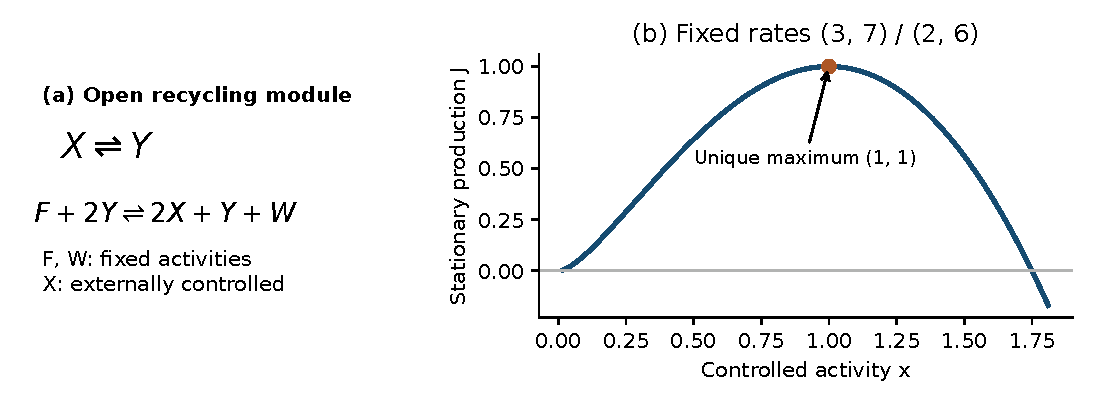
\includegraphics[width=\linewidth]{recycling.pdf}
\caption{The worked recycling source for $m=2$ and its positive stationary production curve for the rates $k^+=(3,7)$, $k^-=(2,6)$. The curve is drawn from the exact stationary equations~\eqref{eq:curve}; the unique global bound $J\le1$ is proved independently by Theorem~\ref{thm:unique}. Activities and time are in the dimensionless model units fixed in the text.}
\label{fig:recycling}
\end{figure}

\begin{figure}[t]
\centering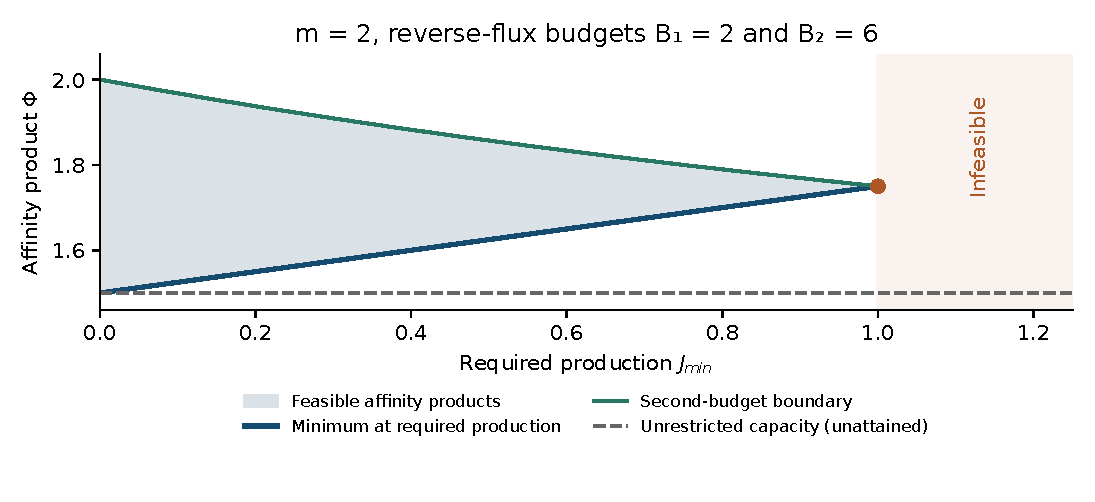
\includegraphics[width=\linewidth]{budgets.pdf}
\caption{Exact two-budget trade-off for $m=2$, $\beta_1=2$, $\beta_2=6$. The shaded region contains the affinity products realizable with production at least the horizontal-axis requirement, between the boundaries~\eqref{eq:rinterval}; the dashed line is the unattained unrestricted capacity $L_2=3/2$. At $\Jmin=\Jmax=1$ only $r=3/2$ and $\Phi=7/4$ remain, and beyond it the budgets are infeasible.}
\label{fig:budgets}
\end{figure}

\subsection{A worked operating point}
Take $m=2$, $\Jmin=1$ and $(\beta_1,\beta_2)=(2,6)$. Then~\eqref{eq:feasible} holds with equality, $\Jmax=1$, the interval~\eqref{eq:rinterval} collapses to $r=3/2$, $q=(3/2,7/6)$, and the reconstruction~\eqref{eq:rates} at the unit reference is $k^+=(3,7)$, $k^-=(2,6)$ with $\Phi=7/4$ instead of the unrestricted $3/2$. Choosing activity units so that the reference is $(x,y)=(1,1)$ and a time unit so that its production is one makes these normalized model values, not measured parameters. The positive stationary curve of this source, shown in Figure~\ref{fig:recycling}, is
\begin{equation}\label{eq:curve}
 x(y)=\frac{-3+\sqrt{9+24y(2y+7y^2)}}{12y},\qquad J(y)=3x(y)-2y,\qquad y>0,
\end{equation}
obtained by solving the stationarity condition $j_1=j_2$ for $x$. The exact linear certificates of Proposition~\ref{prop:budget} are: with $f\ge\one$ and $D(\Jmin)\coloneqq T^{\T}-\Diag(1+\Jmin g_i/\beta_i)$, the vector $(1,3)^{\T}$ is annihilated by $D(1)$, so it is feasible at $\Jmin=1$; and at $\Jmin=6/5$ the nonnegative row $(7/5,1)$ satisfies $(7/5,1)D(6/5)=(-6/25,0)$, so $D(6/5)f\ge0$ with $f\ge\one$ is impossible. Figure~\ref{fig:budgets} shows the whole trade-off.

\begin{proposition}[Attracting controlled operation]\label{prop:stable}
For the rates $k^+=(3,7)$, $k^-=(2,6)$ and $x\equiv1$, every solution of the internal dynamics with $y(0)>0$ exists for all $t\ge0$, stays positive, and converges to $y=1$.
\end{proposition}
\begin{proof}
With $x=1$ the internal equation is
\begin{equation}\label{eq:ode}
 \dot y=j_1-j_2=(3-2y)-(7y^2-6y)=-(y-1)(7y+3),
\end{equation}
positive on $0<y<1$ and negative on $y>1$. By uniqueness of solutions the equilibrium cannot be crossed, so $y(t)$ stays between $y(0)$ and $1$, is monotone, positive and bounded, and converges to a zero of the vector field in that interval, which is $1$. Explicitly, with $c=(y(0)-1)/(7y(0)+3)\in(-1/3,1/7)$,
\[
 y(t)=\frac{1+3ce^{-10t}}{1-7ce^{-10t}},
\]
whose denominator is positive for $t\ge0$. The linearization at the equilibrium is $-10$.
\end{proof}

This is stability with $X$ maintained externally, not autonomous regulation; during transients the controller may have to supply $X$ as well as remove it. A mass-balanced open completion of the module is $X\rightleftharpoons Y$, $F+2Y\rightleftharpoons2X+Y+W$ with fixed food and waste activities $F,W$ absorbed into the coefficients; the masses $m_X=m_Y=m_W=1$, $m_F=2$ balance both reactions. This exhibits a consistent open source, not a specific chemistry: the second reaction is an effective higher-order step, not an elementary mechanism.

\section{Why rootedness and response positivity cannot be conflated}\label{sec:rooted}

The following exact source shows that Theorem~\ref{thm:unique} needs more than rootedness, and that the positive-response capacity is a statement about responses rather than about positive currents.

\subsection{A rooted source with two global maximizers}
Let $X$ be the first species and
\begin{equation}\label{eq:countermatrices}
 \Sp=\begin{pmatrix}0&1&0\\2&1&0\\4&0&1\end{pmatrix},\qquad
 \Sm=\begin{pmatrix}1&0&0\\1&4&0\\1&8&2\end{pmatrix},\qquad
 T=\Sp^{-1}\Sm=\begin{pmatrix}0&2&0\\1&0&0\\1&0&2\end{pmatrix},
\end{equation}
that is, $2Y+4Z\rightleftharpoons X+Y+Z$, $X+Y\rightleftharpoons4Y+8Z$, $Z\rightleftharpoons2Z$. The complexes are nonnegative integers, $\det\Sp=-2$, $\det S=2$, and $g=(3/2,1/2,1/2)^{\T}$ satisfies $Sg=e_X$. The response digraph has edges $1\to2$, $2\to1$, $1\to3$ and $3\to3$ (Figure~\ref{fig:rooted}): it is rooted with terminal component $\{3\}$ and transient component $\{1,2\}$, and not strongly connected. Take $f=(1,1,1)$, so $q=(2,2,2)$, and $J_0=1$: the reconstruction is $k^+=(3,1,1)$, $k^-=(3/2,1/2,1/2)$.

Put $p_i=z^{(\Sp)_i}=e^{\xi_i}$, so $p=(y^2z^4,\,xy,\,z)$, and let $t$ be the normalized production. The stationary equations $C_i(\xi)=t$ read
\begin{equation}\label{eq:tworoots}
 p_2p_3=2p_1-t,\qquad p_1^2=2p_2-t,\qquad p_3^2=2p_3-t .
\end{equation}
The last equation gives $t=1-(p_3-1)^2\le1$, which is Theorem~\ref{thm:global} by hand. At $t=1$: $p_3=1$, $p_2=2p_1-1$, and $p_1^2=4p_1-3$, i.e.\ $(p_1-1)(p_1-3)=0$. There are exactly two positive global maximizers,
\begin{equation}\label{eq:states}
 (x,y,z)=(1,1,1)\qquad\text{and}\qquad(x,y,z)=\big(5/\sqrt3,\ \sqrt3,\ 1\big),
\end{equation}
both with production $1$. Rootedness does not imply uniqueness, and the equality propagation of Lemma~\ref{lem:equality} stops exactly where it should: the zero at $\xi_3$ does not propagate backwards into the transient component $\{1,2\}$, whose block $T_{CC}=\begin{psmallmatrix}0&2\\1&0\end{psmallmatrix}$ has spectral radius $\sqrt2$ and admits no certificate~\eqref{eq:subcritical}.

The phenomenon is not specific to the profile $(1,1,1)$. For any $f\in\cone(T)$ one has $q_3=2$ and $R\coloneqq q_1q_2=2(1+f_3/f_2)>2$, and at $t=1$ the equations factor as $(p_1-1)\big(p_1-(R-1)\big)=0$, with the second root $p=\big(R-1,\ 1+q_1(R-2),\ 1\big)>0$ distinct from $\one$. By Corollary~\ref{cor:arbitrary} every positive-response realization of this source, at any reference state, has a second global maximizer: the unique-global value set is empty, $\Vuniq=\emptyset\ne\Vglob=\Vresp$. This is an empty realization class, not a finite gap between two nonempty capacities.

\begin{figure}[t]
\centering
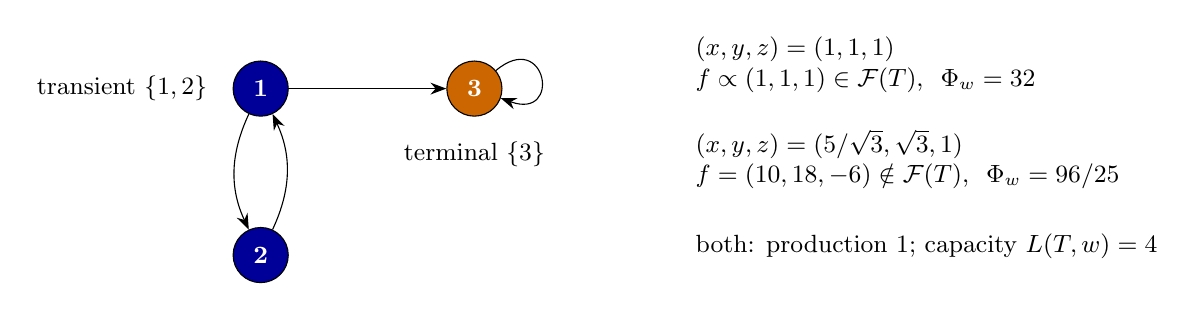
\begin{tikzpicture}[>={Stealth[length=2mm]},node distance=14mm,
 v/.style={circle,draw,fill=blue!60!black,text=white,font=\bfseries\small,minimum size=7mm,inner sep=0pt},
 term/.style={v,fill=orange!80!black}]
\node[v] (1) {1};
\node[v] (2) [below=of 1] {2};
\node[term] (3) [right=20mm of 1] {3};
\draw[->] (1) to[bend right=25] (2);
\draw[->] (2) to[bend right=25] (1);
\draw[->] (1) -- (3);
\draw[->] (3) to[out=40,in=-20,looseness=6] (3);
\node[below=2mm of 3,font=\small] {terminal $\{3\}$};
\node[left=2mm of 1,font=\small] {transient $\{1,2\}$};
\begin{scope}[xshift=54mm,yshift=-7mm]
\node[anchor=west,align=left,font=\small] at (0,10mm) {$(x,y,z)=(1,1,1)$\\ $f\propto(1,1,1)\in\cone(T)$, $\ \Phi_w=32$};
\node[anchor=west,align=left,font=\small] at (0,-2mm) {$(x,y,z)=(5/\sqrt3,\sqrt3,1)$\\ $f=(10,18,-6)\notin\cone(T)$, $\ \Phi_w=96/25$};
\node[anchor=west,align=left,font=\small] at (0,-13mm) {both: production $1$; capacity $L(T,w)=4$};
\end{scope}
\end{tikzpicture}
\caption{The rooted response digraph of the source~\eqref{eq:countermatrices} and its two global maximizers for $w=(3,1,1)$. Only the first has a positive forward response; the affinity product below the capacity at the second does not contradict Theorem~\ref{thm:capacity}.}
\label{fig:rooted}
\end{figure}

\subsection{Positive currents are not positive responses}
Take $w=(3,1,1)=2g$. On the cone $\Phi_w=2q_1^3q_2>4$, and $f=(1,1,\eps)$ gives $\Phi_w=4(1+\eps)^3\to4$, so $L(T,w)=4$, unattained. At the second maximizer the one-way ratios are $(6/5,10/9,2)$ and
\[
 \Phi_w=(6/5)^3\cdot(10/9)\cdot2=96/25<4 .
\]
There is no contradiction. The stationary set through the second state is a regular curve (its reduced internal Jacobian is nonsingular), and its logarithmic tangent is $u=(1,17,-6)$, so the forward response there is $f=\Sp^{\T}u=(10,18,-6)$, which has a negative entry and lies outside $\cone(T)$; the current Jacobian annihilates $u$ as required. All net currents at that state are positive (they equal $g$), but the third forward flux \emph{decreases} with the control. The capacity theorem constrains optima in the forward regime, and positive net currents do not place an optimum there. The response signs are therefore part of the hypothesis, not a convenience.

\subsection{A global maximizer that is a saddle}
The two maximizers~\eqref{eq:states} do not exhibit bistability at one controlled activity, since their controlled activities differ. At the unit state with $x$ held fixed, the internal dynamical Jacobian of $(\dot y,\dot z)$ is
\begin{equation}\label{eq:saddle}
 \Dint=\begin{pmatrix}-15/2&-45/2\\-43/2&-127/2\end{pmatrix},\qquad\det\Dint=-\tfrac{15}{2}<0,
\end{equation}
a saddle. In contrast with Proposition~\ref{prop:stable}, a regular global production optimum need not be dynamically attracting. Stationary production and dynamical stability are separate questions, and the response data fix only the first.

\section{Discussion}\label{sec:discussion}

\paragraph{What the theorem says.}
On the nonnegative-response class the first-order response of a mass-action autocatalytic source at a critical point determines its maximal stationary production, over the whole positive fiber. The mechanism is not a maximum principle for a linear operator but a comparison at a single reaction, made possible because reaction log-coordinates turn fixed monomial kinetics into the two-exponential form~\eqref{eq:normalized}. Rootedness enters only through the regular branch, and strong connectivity (or a subcritical certificate on the transient components) only through uniqueness. The affinity value sets of forward-response profiles, regular local maxima and regular global maxima coincide, and the capacity $L(T,w)$ of~\citep{companion2026}, which is the optimization problem of~\citep[Supplementary Note~11]{despons2024} in response coordinates, is therefore the greatest lower bound of the affinity at global production optima of positive mass-action networks with the given complexes and control, whether or not it is attained.

\paragraph{What it does not say.}
The class is square (as many reactions as species), with one controlled species, invertible $\Sp$ and $S$, positive mode and nonnegative $T$. Nonsquare or overlapping assemblies, several controlled species, or signed response matrices are outside it; the companion paper's interacting-core examples show that nothing can be expected to transfer automatically. Within the class, the theorem concerns stationary production. It does not assert stability (Section~\ref{sec:rooted} shows a global optimum that is a saddle), persistence, bounded molecularity, low-copy behaviour, or a specific biochemical mechanism; Section~\ref{sec:recycling} illustrates the model interpretation, not a fitted pathway. Fixed equilibrium constants alone do not obstruct the realization (Proposition~\ref{prop:fixedK}), but fixed concentration ranges or shared catalyst budgets do restrict it, and~\eqref{eq:budgetcone} is the exact form of one such restriction.

\paragraph{Open problems.}
(i) Theorem~\ref{thm:subcritical} is sufficient for uniqueness; an exact criterion for reducible rooted digraphs remains open, and the source of Section~\ref{sec:rooted} is the smallest failure we know. (ii) The signed-response case: when $T$ has negative entries the minimum comparison~\eqref{eq:minimum} fails, and it is not known whether some other comparison recovers globality on a subclass. (iii) The constrained capacity $L_\beta$: the bound~\eqref{eq:budgetlower} is attained in the recycling family whenever the budgets are consistent, but a general attainment or approximation theory for polyhedral subcones of $\cone(T)$ is not developed here. (iv) Dynamical selection among several global maximizers, and the relation between the routing matrix $P$ of Theorem~\ref{thm:local} and the stability of the controlled dynamics.

\section{Formal verification}\label{sec:formal}

\subsection{Roots and receipts}
The theorems of Sections~\ref{sec:global} and~\ref{sec:capacity} were developed together with a formalization in Lean~4 (toolchain \texttt{leanprover/lean4:v4.30.0}) against a frozen Mathlib manifest, compiled with warnings treated as errors and checked to use no \texttt{sorry} and no axioms beyond \texttt{propext}, \texttt{Classical.choice} and \texttt{Quot.sound}. The development extends the companion paper's library \texttt{OptimalAffinityRealizability}~\citep{companion2026}, whose local-realization theorem is a compiled dependency. Table~\ref{tab:receipts} lists the two root files and the SHA-256 prefixes of their sources at verification time.

\begin{table}[t]
\centering\small
\begin{tabular}{@{}>{\raggedright\arraybackslash}p{0.27\textwidth}>{\raggedright\arraybackslash}p{0.47\textwidth}l@{}}
\toprule
Root file & Exported declarations & SHA-256 prefix \\
\midrule
\texttt{Global\allowbreak Resolution.lean} &
\lean{sharpGlobalResponseCapacityResolution}, \lean{rootedSource_globalCapacityEquality}, \lean{stronglyConnectedSource_uniqueGlobalCapacityEquality}, \lean{rawSquareSource_globalNearCapacity}, \lean{arbitraryRateSource_globalMaximum} &
\texttt{46d42475} \\[2pt]
\texttt{Operating\allowbreak Consequences.lean} &
\lean{fixedEquilibrium_logReference}, \lean{fixedEquilibrium_rateRatio}, \lean{reverseBudget_iff_ratio}, \lean{recycling_twoBudget_feasible_iff}, \lean{recycling_capacity_gap_turnover}, \lean{recycling_controlled_sign} &
\texttt{f7253d7e} \\
\bottomrule
\end{tabular}
\caption{Root files in \texttt{proofs/OptimalAffinityRealizability/} and their exported declarations (namespace \texttt{OptimalAffinityRealizability}). Both receipts record Lean 4.30.0, the same Mathlib manifest (SHA-256 prefix \texttt{a8df0b60}), exit code $0$, empty error output, warnings as errors, and the three standard axioms.}
\label{tab:receipts}
\end{table}

The source is the record \texttt{SquareSource} of the companion library (real nonnegative complex matrices, positive rates, a controlled index, and invertibility of $\Sp$ and $S$ as \texttt{IsUnit} of the determinants), and \texttt{ControlledProductionMode source g} is $Sg=e_X$. The response matrix, cone and objective are \texttt{responseMatrix}, \texttt{ResponseFeasible} and \texttt{responseObjective} with natural-number weights. The primitive source-facing theorem is
\begin{lstlisting}
def ResponseRooted (T : Matrix ι ι ℝ) : Prop :=
  ∃ root, ∀ i, Relation.ReflTransGen (fun a b => 0 < T b a) i root

theorem rootedSource_globalCapacityEquality {n : ℕ} [Nonempty (Fin n)]
    (source : SquareSource n) (weights : Fin n → ℕ) (J : ℝ) (g : Fin n → ℝ)
    (hroot : ResponseRooted (responseMatrix source))
    (hT : ∀ i j, 0 ≤ responseMatrix source i j)
    (hJ : 0 < J) (hg : ∀ i, 0 < g i) (hmode : ControlledProductionMode source g)
    (hne : ∃ f, ResponseFeasible (responseMatrix source) f) :
    (∃ f, GlobalRealizable source J g f) ∧
    realizationCapacity (responseMatrix source) weights (GlobalRealizable source J g) =
      responseLayerCapacity (responseMatrix source) weights
\end{lstlisting}
and the strongly connected variant \texttt{stronglyConnectedSource\_\allowbreak uniqueGlobal\allowbreak Capacity\allowbreak Equality} replaces \texttt{hroot} by \texttt{ResponseStronglyConnected} and \texttt{GlobalRealizable} by \texttt{UniqueGlobalRealizable}. Here \texttt{GlobalRealizable source J g f} is the existence of a record containing the companion paper's strict-local witness (the response ratios, the common tangent, the left null vector $\lambda$ and the regular-branch certificate) together with the proposition that the controlled flux is at most $J$ at every $\zeta\in\R^n$ satisfying the noncontrolled stationary equations of the reconstruction; \texttt{UniqueGlobalRealizable} adds that equality forces $\zeta=0$. The capacities are \texttt{sInf} of the corresponding value sets, so the equalities hold as equalities of real numbers with Mathlib's convention $\inf\emptyset=0$; the hypothesis \texttt{hne} is the nonemptiness of the cone. The root \lean{sharpGlobalResponseCapacityResolution} is the conjunction of the rooted and strongly connected statements over the companion paper's class predicate, and \lean{responseRooted_accessibleRootedClass} proves that graph rootedness with $T\ge0$ and $g>0$ implies that predicate, using \lean{positiveProduction_controlAccessible} for Lemma~\ref{lem:access}.

\subsection{Concordance}
Table~\ref{tab:concordance} maps the statements of this paper to compiled declarations.

\begin{table}[t]
\centering\small
\begin{tabular}{@{}>{\raggedright\arraybackslash}p{0.34\textwidth}>{\raggedright\arraybackslash}p{0.56\textwidth}@{}}
\toprule
Statement & Declaration(s) \\
\midrule
Lemma~\ref{lem:normalized} & \lean{productLogCoordinates_eq}, \lean{reconstructedCurrent_normalized}, \lean{stationary_commonResponseCurrent} \\
Lemma~\ref{lem:scalar} & \lean{exp_tangent_gap_nonneg}, \lean{exp_tangent_gap_eq_zero_iff} \\
Lemma~\ref{lem:minimum} & \lean{responseMinimum_comparison}, \lean{responseMinimum_current_le_one} \\
Theorem~\ref{thm:global} & \lean{commonResponseCurrent_le_one}, \lean{reconstructedSource_globalMaximum} \\
Lemma~\ref{lem:equality} & \lean{commonResponseCurrent_one_nonnegative}, \lean{commonResponseCurrent_zero_propagates} \\
Theorem~\ref{thm:unique} & \lean{commonResponseCurrent_one_eq_zero}, \lean{reconstructedSource_uniqueGlobal} \\
Corollary~\ref{cor:arbitrary}, comparison step & \lean{actualLogCurrent_at_reference}, \lean{arbitraryRateSource_globalMaximum} \\
Lemma~\ref{lem:access} & \lean{controlCovector_eq_productionWeightedResponseGap}, \lean{positiveProduction_controlAccessible} \\
Theorem~\ref{thm:local} & \lean{accessibleRootedResponseClass_rayStrictLocal} (companion library) \\
Theorem~\ref{thm:capacity}, rooted case & \lean{globalValueSet_eq_localValueSet}, \lean{rawSquareSource_globalValueSetEquality}, \lean{rootedSource_globalCapacityEquality} \\
Theorem~\ref{thm:capacity}, strongly connected case & \lean{rawSquareSource_uniqueGlobalValueSetEquality}, \lean{stronglyConnectedSource_uniqueGlobalCapacityEquality} \\
Corollary~\ref{cor:near} & \lean{rawSquareSource_globalNearCapacity} \\
Proposition~\ref{prop:fixedK}, \eqref{eq:Kstate} and the ratio $K_i$ & \lean{fixedEquilibrium_logReference}, \lean{fixedEquilibrium_rateRatio} \\
Proposition~\ref{prop:budget}, scalar equivalence & \lean{reverseBudget_iff_ratio} \\
Eqs.~\eqref{eq:rinterval}--\eqref{eq:feasible} & \lean{recycling_twoBudget_feasible_iff} \\
Eq.~\eqref{eq:inversegap} & \lean{recycling_capacity_gap_turnover} \\
Signs of the vector field~\eqref{eq:ode} & \lean{recycling_controlled_vectorfield}, \lean{recycling_controlled_sign} \\
\bottomrule
\end{tabular}
\caption{Concordance between the paper and the compiled development.}
\label{tab:concordance}
\end{table}

\subsection{What is proved conventionally}\label{subsec:notformal}
The following statements are proved in the text and are not represented by compiled theorem statements; a reader relying on the machine-checked development should be aware of them.
\begin{enumerate}[label=(\arabic*)]
\item Theorem~\ref{thm:subcritical} (uniqueness with subcritical transient components) and Remark~\ref{rem:subcritical}. The compiled uniqueness theorem is the strongly connected case.
\item The derivative-balance step of Corollary~\ref{cor:arbitrary}: the compiled \lean{arbitraryRateSource_globalMaximum} takes the ratio hypothesis~\eqref{eq:ratiohyp} at an actual positive stationary state as input and translates the full state space; it does not itself differentiate an externally specified branch.
\item In Proposition~\ref{prop:fixedK}, the transfer of regularity, curvature and global maximality under the translation $z=z^*\odot y$, and Corollary~\ref{cor:concentration}. The compiled parts are the unique solution of~\eqref{eq:Kstate} and the scalar ratio identity $k^+_i/k^-_i=K_i$.
\item In Proposition~\ref{prop:budget}, the passage from the compiled scalar equivalence to the cone~\eqref{eq:budgetcone}, and the constrained-capacity inequality~\eqref{eq:budgetlower}.
\item In Section~\ref{sec:recycling}, the formulas~\eqref{eq:recycle}, \eqref{eq:minphi}, \eqref{eq:maxJ}, the curve~\eqref{eq:curve}, the linear certificates, and the convergence statement of Proposition~\ref{prop:stable} beyond the compiled signs of the vector field.
\item Section~\ref{sec:rooted} in its entirety: the two maximizers, the second root for every profile, the response $(10,18,-6)$ at the second state, and the Jacobian~\eqref{eq:saddle}. These are exact rational and symbolic computations, reproduced independently by the script described below, and are not a compiled source-level countertheorem.
\end{enumerate}
Exact preflight computations (forty-four exact maximizing-state checks over twenty-two feasible profiles, four thousand sampled comparisons in dimensions two to six with zero excess over the bound, and a deliberately signed-off-diagonal ablation in which the ordering step fails) were used to select the theorems and are not part of any proof.

\subsection{Reproducibility}
The source package of this paper contains the manuscript, the bibliography, the two vector figures, and a script \texttt{check\_paper.py} that re-derives in exact rational and symbolic arithmetic every number printed above: the recycling formulas and worked point, the fixed-$K$ example, the two linear certificates, the explicit solution of~\eqref{eq:ode}, the matrices and both maximizers of~\eqref{eq:countermatrices}, the second root for a general profile, the response at the second state, the Jacobian~\eqref{eq:saddle}, and the spectral radius of the transient block. The Lean sources, the verification receipts, and the exact reproduction commands are recorded in the project repository alongside the companion paper's development.

\bibliographystyle{plainnat}
\bibliography{refs}

\end{document}
